\documentclass{beamer}
\usepackage[utf8]{inputenc}

\usetheme{Madrid}
\usecolortheme{default}
\usepackage{amsmath,amssymb,amsfonts,amsthm}
\usepackage{txfonts}
\usepackage{tkz-euclide}
\usepackage{listings}
\usepackage{adjustbox}
\usepackage[T1]{fontenc}
\usepackage{array}
\usepackage{tabularx}
\usepackage{gvv}
\usepackage{lmodern}
\usepackage{circuitikz}
\usepackage{tikz}
\usepackage{graphicx}

\setbeamertemplate{page number in head/foot}[totalframenumber]

\usepackage{tcolorbox}
\tcbuselibrary{minted,breakable,xparse,skins}



\definecolor{bg}{gray}{0.95}
\DeclareTCBListing{mintedbox}{O{}m!O{}}{%
  breakable=true,
  listing engine=minted,
  listing only,
  minted language=#2,
  minted style=default,
  minted options={%
    linenos,
    gobble=0,
    breaklines=true,
    breakafter=,,
    fontsize=\small,
    numbersep=8pt,
    #1},
  boxsep=0pt,
  left skip=0pt,
  right skip=0pt,
  left=25pt,
  right=0pt,
  top=3pt,
  bottom=3pt,
  arc=5pt,
  leftrule=0pt,
  rightrule=0pt,
  bottomrule=2pt,
  toprule=2pt,
  colback=bg,
  colframe=orange!70,
  enhanced,
  overlay={%
    \begin{tcbclipinterior}
    \fill[orange!20!white] (frame.south west) rectangle ([xshift=20pt]frame.north west);
    \end{tcbclipinterior}},
  #3,
}
\lstset{
    language=C,
    basicstyle=\ttfamily\small,
    keywordstyle=\color{blue},
    stringstyle=\color{orange},
    commentstyle=\color{green!60!black},
    numbers=left,
    numberstyle=\tiny\color{gray},
    breaklines=true,
    showstringspaces=false,
}
%------------------------------------------------------------
%This block of code defines the information to appear in the
%Title page
\title %optional
{ 4.8.14}

%\subtitle{A short story}

\author % (optional)
{Hemanth Reddy-AI25BTECH11018}



\begin{document}


\frame{\titlepage}
\begin{frame}{Question}
Find the position vector of the foot of perpendicular and the perpendicular distance from the point  $ \vec{P}$ with position vector $2\hat{i}  + 3  \hat{j}  + \hat{k} $ to the plane    \textbf{r} $\cdot$ ($ 2\hat{i}  +   \hat{j}  + 3\hat{k}$) -26 = 0.
 Also find image of $ \vec{P}$  in the plane.
\end{frame}



\begin{frame}{Theoretical Solution}
\textbf{Solution:}\\

\begin{align}
   \text{ The position vector of point }  \vec{P} \text{ is }
  \textbf{p} = \myvec{ 2 \\ 3 \\ 1 } 
\end{align}
 The normal vector of the plane is 
\begin{align}
    \textbf{n} = \myvec{ 2 \\ 1 \\ 3 }
\end{align}



The plane equation is
\begin{align}
    \textbf{p}^T \cdot \textbf{n} - 26 = 0
\end{align} \\



\end{frame}

\begin{frame}{Theoretical Solution}

1. Perpendicular Distance\\

The dot product $\textbf{p} \cdot \textbf{n}$ is given by the matrix multiplication $\textbf{p}^T \textbf{n}$.\\

\begin{align}
    \textbf{p}^{T} \textbf{n} = \myvec{ 2 & 3 & 1 } \myvec{ 2 \\ 1 \\ 3 } = (2)(2) + (3)(1) + (1)(3) = 10
\end{align}
 

\begin{align}
    |\textbf{n}| = \sqrt{\textbf{n}^T \textbf{n}} = \sqrt{\myvec{ 2 & 1 & 3 } \myvec{ 2 \\ 1 \\ 3 }} = \sqrt{4+1+9} = \sqrt{14}
\end{align}
The perpendicular distance d is:
\begin{align}
    d = \frac{|\textbf{p}^T \textbf{n} - 26|}{|\textbf{n}|} = \frac{|10-26|}{\sqrt{14}} = \frac{16}{\sqrt{14}}
\end{align}

\end{frame}

\begin{frame}{Theoretical Solution}


2. Foot of Perpendicular\\

The position vector of the foot of the perpendicular    $\textbf{q}$ is:

\begin{align}
    \textbf{q} = \textbf{p} - \frac{(\textbf{p}^T \textbf{n} - 26)}{|\textbf{n}|^2} \textbf{n}
\end{align}
\begin{align}
  \textbf{q}  = \myvec{ 2 \\ 3 \\ 1 } - \frac{10 - 26}{14} \myvec{ 2 \\ 1 \\ 3 } = \myvec{ 2 \\ 3 \\ 1 } + \frac{16}{14} \myvec{ 2 \\ 1 \\ 3 }
\end{align}


\begin{align}
    \textbf{q} = \myvec{ 2 \\ 3 \\ 1 } + \frac{8}{7} \myvec{ 2 \\ 1 \\ 3 } = \myvec{ 2 + 16/7 \\ 3 + 8/7 \\ 1 + 24/7 } = \myvec{ 30/7 \\ 29/7 \\ 31/7 }
\end{align}


So the position vector of the foot of the perpendicular is $\frac{30}{7}\hat{i} + \frac{29}{7}\hat{j} + \frac{31}{7}\hat{k}$.






\end{frame}

\begin{frame}{Theoretical Solution}

3. Image of $ \vec{P}$\\

The position vector of the image $\textbf{P'}$, is:\\

\begin{align}
     \textbf{P'} = 2\textbf{q} - \textbf{P} = 2 \myvec{ 30/7 \\ 29/7 \\ 31/7 } - \myvec{ 2 \\ 3 \\ 1 } = \myvec{ 60/7 - 14/7 \\ 58/7 - 21/7 \\ 62/7 - 7/7 } = \myvec{ 46/7 \\ 37/7 \\ 55/7 }
\end{align}

So the position vector of the image is $\frac{46}{7}\hat{i} + \frac{37}{7}\hat{j} + \frac{55}{7}\hat{k}$.




\end{frame}




\begin{frame}[fragile]
    \frametitle{C Code }
    \begin{lstlisting}

#include <stdio.h>
#include <math.h>

int main() {
  
    double p[3] = {2.0, 3.0, 1.0};
    double n[3] = {2.0, 1.0, 3.0};
    double d0 = 26.0;

    // --- 1. Perpendicular Distance ---
    
   
    double dot_product_pn = 0.0;
    for (int i = 0; i < 3; i++) {
        dot_product_pn += p[i] * n[i];
    }

    
   

    \end{lstlisting}
\end{frame}

\begin{frame}[fragile]
    \frametitle{C Code }
    \begin{lstlisting}

    
 double magnitude_n_sq = 0.0;
    for (int i = 0; i < 3; i++) {
        magnitude_n_sq += n[i] * n[i];
    }
    double magnitude_n = sqrt(magnitude_n_sq);

   
    double distance = fabs(dot_product_pn - d0) / magnitude_n;
    printf("Perpendicular Distance: %.2f / %.2f = %.4f\n\n", fabs(dot_product_pn - d0), magnitude_n, distance);

    // --- 2. Foot of Perpendicular ---
    double scalar_factor = (dot_product_pn - d0) / magnitude_n_sq;
    double q[3];

   
    





    \end{lstlisting}
\end{frame}


\begin{frame}[fragile]
    \frametitle{C Code}
    \begin{lstlisting}

for (int i = 0; i < 3; i++) {
        q[i] = p[i] - scalar_factor * n[i];
    }
    printf("Position vector of Foot of Perpendicular (Q):\n");
    printf("(%.4f, %.4f, %.4f)\n\n", q[0], q[1], q[2]);

    // --- 3. Image of P ---
    double p_prime[3];
    for (int i = 0; i < 3; i++) {
        p_prime[i] = 2.0 * q[i] - p[i];
    }
    printf("Position vector of Image of P (P'):\n");
    printf("(%.4f, %.4f, %.4f)\n\n", p_prime[0], p_prime[1], p_prime[2]);
    return 0;
}


    \end{lstlisting}
\end{frame}


\begin{frame}[fragile]
    \frametitle{Python Code}
    \begin{lstlisting}

import numpy as np
import matplotlib.pyplot as plt
from mpl_toolkits.mplot3d import Axes3D

n = np.array([2, 1, 3])  # Normal vector to the plane
p = np.array([2, 3, 1])  # Position vector of point P
d = 26  # Plane constant

# Calculate the foot of perpendicular from P to the plane
t_foot = (d - np.dot(n, p)) / np.dot(n, n)
foot = p + t_foot * n

# Calculate image of P (reflection about the plane)
image = 2 * foot - p

# Create grid for the plane
xx, yy = np.meshgrid(np.linspace(0, 8, 8), np.linspace(0, 8, 8))
zz = (d - 2 * xx - yy) / 3




    \end{lstlisting}
\end{frame}


\begin{frame}[fragile]
    \frametitle{Python Code}
    \begin{lstlisting}


# Plotting
fig = plt.figure(figsize=(10, 8))
ax = fig.add_subplot(111, projection='3d')
ax.plot_surface(xx, yy, zz, alpha=0.6, color='cyan', rstride=1, cstride=1, edgecolor='none')

# Plot point P, foot of perpendicular, and image
ax.scatter(*p, color='blue', s=80, label='P (2,3,1)')
ax.scatter(*foot, color='red', s=80, label='Foot of Perpendicular')
ax.scatter(*image, color='green', s=80, label='Image of P')

# Plot perpendicular line
ax.plot([p[0], foot[0]], [p[1], foot[1]], [p[2], foot[2]], color='black', lw=2, linestyle='--', label='Perpendicular')





    \end{lstlisting}
\end{frame}

\begin{frame}[fragile]
    \frametitle{Python Code}
    \begin{lstlisting}

ax.set_xlim(0, 8)
ax.set_ylim(0, 8)
ax.set_zlim(0, 8)

ax.set_xlabel('X axis')
ax.set_ylabel('Y axis')
ax.set_zlabel('Z axis')
ax.set_title('3D Solution Graph: Foot, Distance, Image')
ax.legend()

plt.tight_layout()
plt.savefig('3d_plane_solution.png')
plt.show()
    \end{lstlisting}
\end{frame}
  
\begin{frame}{Plot}

\begin{figure}
    \centering
    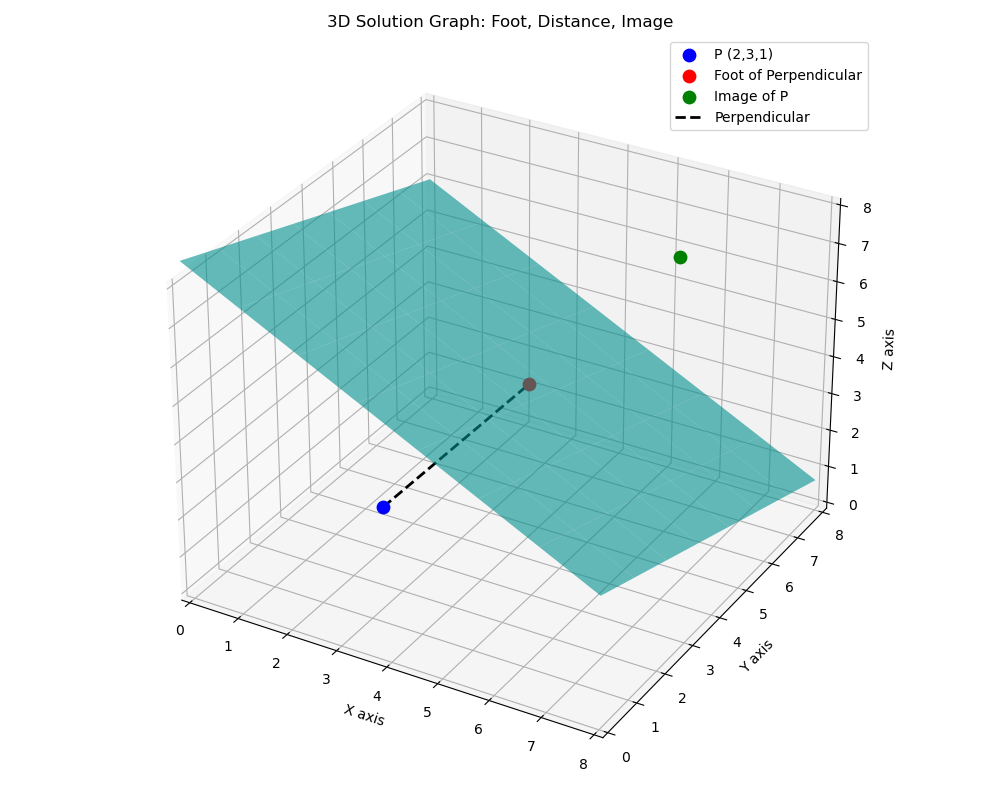
\includegraphics[width=0.8\linewidth]{Beamer/figs/3d_plane_solution.png}
    \caption{}
    \label{fig:placeholder}
\end{figure}

\end{frame}




\end{document}




